\documentclass[conference]{IEEEtran}
\IEEEoverridecommandlockouts
\usepackage[T1]{fontenc}
\usepackage{cite}
\usepackage{amsmath}
\usepackage{newtxtext,newtxmath}
\usepackage{graphicx}
\usepackage{textcomp}
\usepackage{xcolor}
\usepackage{booktabs}
\usepackage{url}
\usepackage{siunitx}
\usepackage[hidelinks]{hyperref}
\graphicspath{{figures/}}
% AUTO-GENERATED by src/analyze.py - do not edit by hand
\newcommand{\accMlp}{59.29}
\newcommand{\accsdMlp}{0.20}
\newcommand{\accsmallMlp}{45.01}
\newcommand{\foneMlp}{58.93}
\newcommand{\aucMlp}{92.22}
\newcommand{\ttrainMlp}{30.6}
\newcommand{\egpuMlp}{0.59}
\newcommand{\etotMlp}{1.81}
\newcommand{\whMlp}{0.50}
\newcommand{\coMlp}{0.24}
\newcommand{\pavgMlp}{19.4}
\newcommand{\utilMlp}{33}
\newcommand{\vramMlp}{46}
\newcommand{\vramnvmlMlp}{643}
\newcommand{\vramtheoMlp}{45}
\newcommand{\vraminfMlp}{48}
\newcommand{\ramMlp}{835}
\newcommand{\tflopsMlp}{0.56}
\newcommand{\tinfMlp}{15}
\newcommand{\einfMlp}{0.9}
\newcommand{\einfimgMlp}{0.090}
\newcommand{\thrMlp}{690.2}
\newcommand{\latMlp}{1.30}
\newcommand{\cpumsMlp}{0.186}
\newcommand{\speedupMlp}{125}
\newcommand{\paramsMlp}{3.81}
\newcommand{\macsMlp}{3.8}
\newcommand{\actsMlp}{5}
\newcommand{\btMlp}{1.041}
\newcommand{\beMlp}{0.905}
\newcommand{\rtMlp}{0.9613}
\newcommand{\tpseMlp}{40.8}
\newcommand{\epseMlp}{0.787}
\newcommand{\accSmall}{81.11}
\newcommand{\accsdSmall}{0.19}
\newcommand{\accsmallSmall}{40.40}
\newcommand{\foneSmall}{81.02}
\newcommand{\aucSmall}{97.98}
\newcommand{\ttrainSmall}{28.8}
\newcommand{\egpuSmall}{0.90}
\newcommand{\etotSmall}{2.11}
\newcommand{\whSmall}{0.59}
\newcommand{\coSmall}{0.28}
\newcommand{\pavgSmall}{32.6}
\newcommand{\utilSmall}{36}
\newcommand{\vramSmall}{40}
\newcommand{\vramnvmlSmall}{635}
\newcommand{\vramtheoSmall}{34}
\newcommand{\vraminfSmall}{153}
\newcommand{\ramSmall}{953}
\newcommand{\tflopsSmall}{0.99}
\newcommand{\tinfSmall}{48}
\newcommand{\einfSmall}{3.9}
\newcommand{\einfimgSmall}{0.394}
\newcommand{\thrSmall}{209.4}
\newcommand{\latSmall}{1.07}
\newcommand{\cpumsSmall}{0.157}
\newcommand{\speedupSmall}{33}
\newcommand{\paramsSmall}{0.55}
\newcommand{\macsSmall}{6.1}
\newcommand{\actsSmall}{115}
\newcommand{\btSmall}{0.954}
\newcommand{\beSmall}{0.949}
\newcommand{\rtSmall}{0.9628}
\newcommand{\tpseSmall}{38.5}
\newcommand{\epseSmall}{1.196}
\newcommand{\accMedium}{90.61}
\newcommand{\accsdMedium}{0.23}
\newcommand{\accsmallMedium}{67.72}
\newcommand{\foneMedium}{90.60}
\newcommand{\aucMedium}{99.47}
\newcommand{\ttrainMedium}{62.6}
\newcommand{\egpuMedium}{4.25}
\newcommand{\etotMedium}{6.42}
\newcommand{\whMedium}{1.78}
\newcommand{\coMedium}{0.85}
\newcommand{\pavgMedium}{67.9}
\newcommand{\utilMedium}{81}
\newcommand{\vramMedium}{163}
\newcommand{\vramnvmlMedium}{755}
\newcommand{\vramtheoMedium}{188}
\newcommand{\vraminfMedium}{295}
\newcommand{\ramMedium}{712}
\newcommand{\tflopsMedium}{11.03}
\newcommand{\tinfMedium}{247}
\newcommand{\einfMedium}{18.4}
\newcommand{\einfimgMedium}{1.840}
\newcommand{\thrMedium}{40.4}
\newcommand{\latMedium}{2.20}
\newcommand{\cpumsMedium}{1.744}
\newcommand{\speedupMedium}{70}
\newcommand{\paramsMedium}{1.15}
\newcommand{\macsMedium}{152.8}
\newcommand{\actsMedium}{717}
\newcommand{\btMedium}{1.003}
\newcommand{\beMedium}{0.989}
\newcommand{\rtMedium}{0.9916}
\newcommand{\tpseMedium}{83.5}
\newcommand{\epseMedium}{5.665}
\newcommand{\accMobile}{90.47}
\newcommand{\accsdMobile}{0.12}
\newcommand{\accsmallMobile}{62.58}
\newcommand{\foneMobile}{90.44}
\newcommand{\aucMobile}{99.44}
\newcommand{\ttrainMobile}{292.1}
\newcommand{\egpuMobile}{19.71}
\newcommand{\etotMobile}{30.07}
\newcommand{\whMobile}{8.35}
\newcommand{\coMobile}{3.96}
\newcommand{\pavgMobile}{67.5}
\newcommand{\utilMobile}{63}
\newcommand{\vramMobile}{1245}
\newcommand{\vramnvmlMobile}{1920}
\newcommand{\vramtheoMobile}{886}
\newcommand{\vraminfMobile}{968}
\newcommand{\ramMobile}{884}
\newcommand{\tflopsMobile}{1.41}
\newcommand{\tinfMobile}{901}
\newcommand{\einfMobile}{68.3}
\newcommand{\einfimgMobile}{6.832}
\newcommand{\thrMobile}{11.1}
\newcommand{\latMobile}{13.87}
\newcommand{\cpumsMobile}{5.888}
\newcommand{\speedupMobile}{65}
\newcommand{\paramsMobile}{2.30}
\newcommand{\macsMobile}{91.2}
\newcommand{\actsMobile}{3521}
\newcommand{\btMobile}{1.037}
\newcommand{\beMobile}{1.017}
\newcommand{\rtMobile}{0.9771}
\newcommand{\tpseMobile}{389.4}
\newcommand{\epseMobile}{26.277}
\newcommand{\accRes}{92.25}
\newcommand{\accsdRes}{0.05}
\newcommand{\accsmallRes}{56.70}
\newcommand{\foneRes}{92.24}
\newcommand{\aucRes}{99.63}
\newcommand{\ttrainRes}{196.4}
\newcommand{\egpuRes}{13.21}
\newcommand{\etotRes}{19.97}
\newcommand{\whRes}{5.55}
\newcommand{\coRes}{2.63}
\newcommand{\pavgRes}{67.3}
\newcommand{\utilRes}{91}
\newcommand{\vramRes}{410}
\newcommand{\vramnvmlRes}{1041}
\newcommand{\vramtheoRes}{474}
\newcommand{\vraminfRes}{642}
\newcommand{\ramRes}{897}
\newcommand{\tflopsRes}{12.74}
\newcommand{\tinfRes}{748}
\newcommand{\einfRes}{52.0}
\newcommand{\einfimgRes}{5.197}
\newcommand{\thrRes}{13.4}
\newcommand{\latRes}{6.65}
\newcommand{\cpumsRes}{5.893}
\newcommand{\speedupRes}{79}
\newcommand{\paramsRes}{11.17}
\newcommand{\macsRes}{555.4}
\newcommand{\actsRes}{1417}
\newcommand{\btRes}{0.991}
\newcommand{\beRes}{0.960}
\newcommand{\rtRes}{0.9976}
\newcommand{\tpseRes}{261.8}
\newcommand{\epseRes}{17.620}
\newcommand{\idlepower}{16.7}
\newcommand{\nruns}{100}
\newcommand{\totalhours}{1.57}
\newcommand{\totalwh}{156.7}
\newcommand{\totalco}{74.4}
\newcommand{\totalgpuwh}{100.7}
\newcommand{\rhoflops}{0.60}
\newcommand{\rhoparams}{0.50}
\newcommand{\rlogflops}{0.800}
\newcommand{\rvram}{0.977}
\newcommand{\dacc}{1.63}
\newcommand{\denergy}{8.97}
\newcommand{\kjperpoint}{5.49}
\newcommand{\sharegpu}{64}
\newcommand{\sharecpu}{26}
\newcommand{\shareram}{10}
\newcommand{\ccvsnvml}{1.002}
\newcommand{\cvtime}{8.9}
\newcommand{\cvenergy}{6.2}


\begin{document}

\title{Time, Memory, Energy and Accuracy: An Empirical Complexity Analysis of Five Deep Learning Architectures on CIFAR-10}

\newcommand{\affil}{\textit{Dept. of Software Engineering}\\ \textit{Istanbul Health and Technology University}\\ Istanbul, T{\"u}rkiye}
\author{
\IEEEauthorblockN{Baran Kemal K{\i}l{\i}{\c{c}}}
\IEEEauthorblockA{\affil\\ 240609043}
\and
\IEEEauthorblockN{{\.I}rem Serra Onmaz}
\IEEEauthorblockA{\affil\\ 240609009}
\and
\IEEEauthorblockN{Nihat G{\"u}ney}
\IEEEauthorblockA{\affil\\ 240609050}
\and
\IEEEauthorblockN{S{\"u}leyman Canberk E{\u{g}}riboz}
\IEEEauthorblockA{\affil\\ 240609014}
}

\maketitle

% ============================================================================
\begin{abstract}
Deep learning models are usually compared by accuracy alone, although their training and deployment
costs in time, memory and energy differ by orders of magnitude. This paper presents a controlled,
repeated-measures study of the \emph{multi-dimensional} complexity of five image classifiers of increasing
and qualitatively different computational character---a multi-layer perceptron (MLP), a small CNN, a
VGG-style medium CNN, MobileNetV2 and ResNet-18---trained from scratch on CIFAR-10.
Each model is trained on four stratified training-set sizes (5k to 50k images) with five random seeds
(\nruns{} runs) on a single RTX~4060 Laptop GPU. For training and inference separately we record wall-clock time,
peak RAM and VRAM, GPU energy from the NVML hardware counter, whole-system energy and CO$_2$ from CodeCarbon,
and Accuracy/Precision/Recall/F1/ROC-AUC, and we relate them to the analytical cost of each network
(parameters $P$, multiply--accumulates per image $F$, activations per image $A$).
Training time grows linearly with the data size $n$, as predicted by $\Theta(E\,n\,F)$: the fitted
exponents lie between \btSmall{} and \btMlp{} and every 95\% confidence interval contains~1, while peak VRAM is
independent of $n$. Energy, in contrast, grows slightly \emph{sub}-linearly for some models because the average
power falls during longer runs. Across models FLOPs are a poor predictor of cost: MobileNetV2 needs $6\times$ fewer
MACs than ResNet-18 but trains $1.5\times$ slower, uses $3\times$ more VRAM and $1.5\times$ more energy, because its
depthwise layers are memory-bound (\tflopsMobile{} vs.\ \tflopsRes{} TFLOP/s) and its memory is dominated by the
$B\cdot A$ activation term. ResNet-18 reaches the best accuracy (\accRes\%), but a VGG-style CNN reaches \accMedium\%
with $3.1\times$ less energy, so each extra accuracy point of ResNet-18 costs \kjperpoint\,kJ. We conclude that energy
must be reported as a separate dimension and that arithmetic intensity, depth and fixed per-step overheads, not only
the asymptotic operation count, govern the practical complexity of a network.
\end{abstract}

\begin{IEEEkeywords}
algorithm analysis, computational complexity, energy efficiency, green AI, deep learning, CIFAR-10, carbon footprint, GPU
\end{IEEEkeywords}

% ============================================================================
\section{Introduction}
The cost of an algorithm is traditionally expressed by its asymptotic running time $T(n)$ and space $S(n)$.
For modern artificial intelligence (AI) workloads a third resource has become equally important: energy.
Training a single large model can emit as much CO$_2$ as several cars over their lifetime~\cite{strubell2019energy},
which motivated the ``Green AI'' agenda of reporting efficiency next to accuracy~\cite{schwartz2020green,henderson2020systematic}.
For the energy of a computation the simplest model is
\begin{equation}
E(n) = P_{avg}\cdot T(n),
\label{eq:energy}
\end{equation}
where $P_{avg}$ is the average power drawn while the program runs. Eq.~\eqref{eq:energy} suggests that energy is just
time multiplied by a constant; in practice, however, $P_{avg}$ depends on how intensively the hardware is utilised,
which in turn depends on the algorithm and its memory-access pattern~\cite{akpinar2026dc,penev2024energy}.

This paper studies this question for deep neural networks (DNNs) on a classical image classification benchmark,
CIFAR-10~\cite{krizhevsky2009cifar}. Five architectures that solve the \emph{same} task under the \emph{same}
training protocol are compared along four dimensions---time, space, energy and predictive performance---separately
for training and for inference, and the measurements are confronted with the analytical complexity of each network.
Our contributions are:
\begin{itemize}
\item a reproducible measurement harness (open source) that isolates the model from data-loading overheads and records
time, RAM, VRAM, hardware-counter GPU energy and CodeCarbon CPU/GPU/RAM energy and CO$_2$ for every phase;
\item an analytical complexity model (parameters, MACs and activations obtained with forward hooks) and its
empirical validation through log--log scaling exponents with confidence intervals over \nruns{} runs;
\item evidence that operation count explains scaling \emph{within} a model but not \emph{across} models,
and that peak training memory is governed by activations rather than parameters;
\item a performance--cost trade-off analysis including a Pareto front, the marginal energy price of accuracy,
and GPU versus CPU inference.
\end{itemize}

% ============================================================================
\section{Related Work}
\textbf{Energy of classical algorithms.} Akp{\i}nar \emph{et al.}~\cite{akpinar2026dc} compared MergeSort, QuickSort,
classical and Strassen matrix multiplication with CodeCarbon and showed that energy behaviour depends on the data
distribution and implementation choices, not only on asymptotic complexity. Penev \emph{et al.}~\cite{penev2024energy}
measured time and energy of heuristic search/optimisation algorithms and found large differences between algorithms
that solve the same task. Our study transfers this ``energy as a complexity dimension'' view to DNNs.

\textbf{Energy of AI models.} Yu \emph{et al.}~\cite{yu2022clinical} compared nine inference algorithms on clinical
laboratory data with Intel Power Gadget and showed that the most accurate models are not the most energy-efficient.
Ko{\c{c}} and {\c{C}}etinta{\c{s}}~\cite{koc2025berturk} evaluated three Turkish BERT variants and reported that
the smallest (DistilBERTurk) has the lowest memory, latency and estimated CO$_2$ while the largest is most accurate.
Iyer \emph{et al.}~\cite{iyer2026greenai} profiled pruning and quantisation over nine networks and observed that
compression may even \emph{increase} runtime memory, i.e.\ memory must be treated as an independent constraint.
Strubell \emph{et al.}~\cite{strubell2019energy}, Lacoste \emph{et al.}~\cite{lacoste2019quantifying} and
Patterson \emph{et al.}~\cite{patterson2021carbon} quantified the carbon footprint of training, and
Henderson \emph{et al.}~\cite{henderson2020systematic} argued for systematic reporting of energy.

\textbf{Hardware and deployment.} {\c{C}}etinkaya and Sertba{\c{s}}~\cite{cetinkaya2022gpucpu} trained CNN, RNN and
LSTM models on GPU and CPU and showed that data-set size drives both run time and GPU power. Zhang and
Li~\cite{zhang2023embedded} reviewed AI on resource-constrained embedded devices, where memory and energy rather than
accuracy are the binding constraints. Canziani \emph{et al.}~\cite{canziani2016analysis} showed that accuracy,
operation count, memory and inference time of ImageNet models are only loosely coupled.

\textbf{Gap.} Most studies report a single run, a single data size or only inference. We contribute repeated
measurements (mean$\pm$std over five seeds), four data sizes for empirical scaling exponents, separate training and
inference phases, and an explicit comparison with the analytical complexity of each architecture.

% ============================================================================
\section{Theoretical Background and Complexity Analysis}
\subsection{Cost of the building blocks}
Let a layer receive $C_{in}$ channels and produce $C_{out}$ channels of spatial size $H\times W$ with a $k\times k$
kernel and $g$ groups. The forward multiply--accumulate (MAC) counts and parameter counts are
\begin{align}
\text{MAC}_{conv} &= H W\, C_{out}\, \tfrac{C_{in}}{g}\, k^2, & P_{conv} &= C_{out}\tfrac{C_{in}}{g}k^2, \label{eq:conv}\\
\text{MAC}_{fc} &= d_{in}\, d_{out}, & P_{fc} &= d_{in} d_{out}. \label{eq:fc}
\end{align}
A standard convolution has $g=1$; a depthwise convolution has $g=C_{in}=C_{out}$, which reduces its cost by a factor
$C_{in}$. Batch normalisation~\cite{ioffe2015bn}, ReLU and pooling cost $O(HWC)$ and are negligible in MACs but
not in memory traffic. Summing~\eqref{eq:conv}--\eqref{eq:fc} over all layers gives the forward cost per image $F$;
summing output sizes gives the number of activations per image $A$ that must be stored for back-propagation.

\subsection{Architectures}
\textbf{MLP}: $3072\!\to\!1024\!\to\!512\!\to\!256\!\to\!10$ with BN and ReLU; no weight sharing, hence
$F\approx P$. \textbf{SmallCNN}: two $3\times3$ conv layers (32, 64 filters) with max-pooling and a 128-unit FC layer.
\textbf{MediumCNN}: VGG-style~\cite{simonyan2015vgg} six $3\times3$ conv layers (64--256 filters) with BN and global
average pooling. \textbf{MobileNetV2}~\cite{sandler2018mobilenetv2}: 17 inverted-residual blocks
(expand $1\times1$ $\to$ depthwise $3\times3$ $\to$ project $1\times1$), CIFAR variant with stride~1 in the stem.
\textbf{ResNet-18}~\cite{he2016resnet}: CIFAR variant with a $3\times3$ stem and four stages of two basic blocks.
Table~\ref{tab:complexity} lists the analytically computed $P$, $F$ and $A$.

\begin{table}[t]
\centering
\caption{Analytical complexity per $32\times32$ image (computed with forward hooks)}
\label{tab:complexity}
\begin{tabular}{lrrrr}
\toprule
Model & Params & MACs/img & Act./img & Layers \\
\midrule
MLP & 3.81M & 3.8M & 5K & 4 \\
SmallCNN & 0.55M & 6.1M & 115K & 4 \\
MediumCNN & 1.15M & 152.8M & 717K & 7 \\
MobileNetV2 & 2.30M & 91.2M & 3521K & 58 \\
ResNet18 & 11.17M & 555.4M & 1417K & 21 \\
\bottomrule
\end{tabular}
\end{table}

Two observations follow directly. (i) Parameters and operations are decoupled: the MLP has
$\paramsMlp$M parameters but only $\macsMlp$M MACs, whereas MediumCNN has fewer parameters ($\paramsMedium$M) but
$\macsMedium$M MACs because each convolution weight is reused at every spatial position.
(ii) MobileNetV2 has $6\times$ fewer MACs than ResNet-18 but $\approx2.5\times$ more activations, since its
expansion layers create six-times wider feature maps at high resolution.

\subsection{Time complexity}
With $n$ training images, $E$ epochs and a backward pass that costs roughly twice the forward pass, the training work
and the inference work on $m$ images are
\begin{equation}
W_{train}(n) \approx 3\,F\,n\,E = \Theta(n), \qquad W_{inf}(m) = F\,m = \Theta(m).
\label{eq:time}
\end{equation}
For a fixed architecture and hyper-parameters, training time is therefore \emph{linear} in $n$. Across architectures,
$T\propto F$ holds only if every network attains the same throughput (FLOP/s). According to the roofline
model~\cite{williams2009roofline}, a kernel with low \emph{arithmetic intensity} (FLOPs per byte moved) is bounded
by memory bandwidth rather than by compute: a depthwise $3\times3$ convolution performs only 9 MACs per input value,
compared with $9C_{in}$ for a dense convolution, so it is expected to be memory-bound.

\subsection{Space complexity}
Under mixed-precision training~\cite{micikevicius2018mixed} with SGD and momentum, the training memory is
\begin{equation}
M_{train} \approx \underbrace{3\cdot4P}_{\text{weights, grads, momentum}} + \underbrace{B\,A\,b_{act}}_{\text{stored activations}},
\label{eq:mem}
\end{equation}
with batch size $B$ and $b_{act}=2$ bytes. $M_{train}$ is independent of $n$ ($\Theta(1)$ in the data size, since
mini-batches are streamed) and linear in $P$ and $A$. Inference needs only $4P$ plus the activations of the
current layer, i.e.\ much less memory.

\subsection{Energy}
Combining \eqref{eq:energy} and \eqref{eq:time}, $E_{train}(n)=P_{avg}\,c\,F\,n\,E$ is also $\Theta(n)$, but
$P_{avg}$ is model-dependent: a kernel that keeps the GPU busy draws more power per second but finishes sooner.

\subsection{Hypotheses}
\textbf{H1}: training time and energy scale linearly with $n$ (exponent $b\approx1$).
\textbf{H2}: across models, cost is ordered by $F$ but not proportional to it.
\textbf{H3}: peak training VRAM follows \eqref{eq:mem} and is dominated by $B\,A$, not by $P$.
\textbf{H4}: $P_{avg}$ differs between models, so energy is not a constant multiple of time.
\textbf{H5}: accuracy improves with $F$ and $n$ with diminishing returns per joule.

% ============================================================================
\section{Methodology and Experimental Setup}
\subsection{Data}
CIFAR-10~\cite{krizhevsky2009cifar} contains 60\,000 $32\times32$ RGB images of 10 balanced classes
(50\,000 training, 10\,000 test). The target is the class label (airplane, automobile, bird, cat, deer, dog, frog,
horse, ship, truck). To study scaling we draw \emph{stratified} subsets with fractions
$\{0.1, 0.25, 0.5, 1.0\}$, i.e.\ $n\in\{5\,000, 12\,500, 25\,000, 50\,000\}$, with 10\% per class. The subset is
determined by the seed, so for a given seed every model sees exactly the same images. All models are evaluated on the
full 10\,000-image test set. Inputs are normalised with the per-channel training mean and standard deviation; training
uses random crop (padding 4) and horizontal flip.

\subsection{Training protocol}
All five models share the same protocol: 15 epochs, batch size $B=128$, SGD with Nesterov momentum 0.9,
weight decay $5\cdot10^{-4}$, one-cycle learning-rate schedule~\cite{smith2019onecycle} with peak 0.1, bfloat16
automatic mixed precision and channels-last memory layout in PyTorch~\cite{paszke2019pytorch}. Every
(model, $n$) configuration is repeated with seeds $\{0,\dots,4\}$, giving
$5\times4\times5=\nruns$ runs. The order of models is shuffled within each (seed, $n$) block so that thermal drift of
the laptop does not systematically favour one model, and an unrecorded warm-up run initialises CUDA and cuDNN
auto-tuning. To keep the measurement attributable to the model, the whole data set ($\approx$180\,MB as uint8) is kept
resident in GPU memory and augmentation is vectorised on the GPU, which removes the CPU data loader from the critical path.

\subsection{Measurements}
\textbf{Time}: \texttt{time.perf\_counter} around each phase after \texttt{torch.cuda.synchronize()}.
\textbf{Space}: peak process RSS sampled every 50\,ms with psutil; peak VRAM as the PyTorch allocator peak minus the
memory already allocated for the resident data set (model-attributable), and the NVML device memory in use
(includes the CUDA context).
\textbf{Energy}: GPU energy from the NVML hardware energy counter~\cite{nvml} (millijoule resolution);
CPU, GPU and RAM energy and CO$_2$ from CodeCarbon~3.3.3~\cite{codecarbon} in offline mode with the carbon
intensity of the Turkish grid. On Windows Intel RAPL is not exposed, so CodeCarbon estimates CPU power from CPU load
and TDP; the GPU part is measured. We report $P_{avg}=E/T$ and the idle GPU power (\idlepower\,W) to separate static
from dynamic energy.
\textbf{Inference}: (i) batched GPU inference over the 10k test set with $B=1000$, repeated until at least 3\,s have
elapsed and averaged per pass so that the energy counter has enough resolution; (ii) online latency with $B=1$ over
300 images; (iii) CPU inference (fp32, 14 threads, $B=250$) on 2\,000 images for the full-data models.
\textbf{Performance}: Accuracy, macro Precision, Recall, F1 and one-vs-rest macro ROC-AUC (scikit-learn).

\subsection{Hardware and software}
Table~\ref{tab:hw} lists the environment. The laptop was connected to mains power on the ``High performance'' plan.
All experiments use the same hardware. GPU access was available; CPU numbers are reported for inference only.

\begin{table}[t]
\centering
\caption{Experimental environment}
\label{tab:hw}
\begin{tabular}{ll}
\toprule
CPU & Intel Core i7-12700H (14 C / 20 T)\\
RAM & 32 GB\\
GPU & RTX 4060 Laptop, 8 GB, 100 W\\
OS & Windows 11 Home (26300)\\
Driver/CUDA/cuDNN & 621.24 / 12.4 / 9.1\\
Python / PyTorch & 3.12.10 / 2.6.0\\
Libraries & scikit-learn 1.9.1, CodeCarbon 3.3.3\\
\bottomrule
\end{tabular}
\end{table}

\subsection{Statistical analysis}
For every configuration we report mean $\pm$ standard deviation over five seeds. Scaling exponents are estimated by
least squares on $\log T = \log c + b\log n$ using all 20 runs of a model, with 95\% $t$-confidence intervals.
Differences between models are tested with Welch's $t$-test. All numbers in this paper are generated
automatically from the raw measurement file by the analysis script.

% ============================================================================
\section{Experimental Results and Discussion}
\subsection{Overall results}
Table~\ref{tab:main} summarises training at full data size and Table~\ref{tab:meminf} memory and inference.
The median coefficient of variation across seeds is \cvtime\% for training time and \cvenergy\% for training
energy, so the measurement noise is small compared with the differences between models.

\begin{table*}[t]
\centering
\caption{Training at $n=50\,000$ (mean $\pm$ std over 5 seeds). $E^{GPU}$: NVML hardware counter; $E^{tot}$: CodeCarbon CPU+GPU+RAM}
\label{tab:main}
\begin{tabular}{lccccc}
\toprule
Model & Acc. (\%) & F1 (\%) & $T_{train}$ (s) & $E^{GPU}_{train}$ (kJ) & $E^{tot}_{train}$ (kJ) \\
\midrule
MLP & 59.29 $\pm$ 0.20 & 58.93 $\pm$ 0.18 & 30.6 $\pm$ 2.8 & 0.59 $\pm$ 0.02 & 1.81 $\pm$ 0.10 \\
SmallCNN & 81.11 $\pm$ 0.19 & 81.02 $\pm$ 0.20 & 28.8 $\pm$ 5.8 & 0.90 $\pm$ 0.05 & 2.11 $\pm$ 0.20 \\
MediumCNN & 90.61 $\pm$ 0.23 & 90.60 $\pm$ 0.24 & 62.6 $\pm$ 4.6 & 4.25 $\pm$ 0.32 & 6.42 $\pm$ 0.38 \\
MobileNetV2 & 90.47 $\pm$ 0.12 & 90.44 $\pm$ 0.12 & 292.1 $\pm$ 24.5 & 19.71 $\pm$ 1.40 & 30.07 $\pm$ 2.05 \\
ResNet18 & 92.25 $\pm$ 0.05 & 92.24 $\pm$ 0.05 & 196.4 $\pm$ 6.1 & 13.21 $\pm$ 0.57 & 19.97 $\pm$ 0.47 \\
\bottomrule
\end{tabular}
\end{table*}

\begin{table*}[t]
\centering
\caption{Memory and inference at $n=50\,000$ (mean $\pm$ std). VRAM$_{tr}$: model-attributable peak during training; $T_{inf}$, $E_{inf}$: one pass over the 10k test set on the GPU ($B=1000$)}
\label{tab:meminf}
\begin{tabular}{lccccc}
\toprule
Model & VRAM$_{tr}$ (MB) & RAM$_{tr}$ (MB) & $T_{inf}$ (ms) & $E_{inf}$ (J) & Lat.$_{B=1}$ (ms) \\
\midrule
MLP & 46 $\pm$ 0 & 835 $\pm$ 588 & 15 $\pm$ 3 & 0.9 $\pm$ 0.1 & 1.30 $\pm$ 0.37 \\
SmallCNN & 40 $\pm$ 2 & 953 $\pm$ 841 & 48 $\pm$ 3 & 3.9 $\pm$ 0.1 & 1.07 $\pm$ 0.36 \\
MediumCNN & 163 $\pm$ 1 & 712 $\pm$ 608 & 247 $\pm$ 4 & 18.4 $\pm$ 1.0 & 2.20 $\pm$ 0.59 \\
MobileNetV2 & 1245 $\pm$ 1 & 884 $\pm$ 695 & 901 $\pm$ 2 & 68.3 $\pm$ 1.7 & 13.87 $\pm$ 3.42 \\
ResNet18 & 410 $\pm$ 0 & 897 $\pm$ 672 & 748 $\pm$ 8 & 52.0 $\pm$ 1.5 & 6.65 $\pm$ 1.84 \\
\bottomrule
\end{tabular}
\end{table*}

\subsection{Scaling with the data size (H1)}
Fig.~\ref{fig:time} and Fig.~\ref{fig:energy} show training time and GPU energy versus $n$ on log--log axes;
Table~\ref{tab:scaling} gives the fitted exponents. All five time exponents are statistically indistinguishable from
one (ResNet-18: $b_T=\btRes$, $R^2=\rtRes$; MediumCNN: $b_T=\btMedium$; MobileNetV2: $b_T=\btMobile$; MLP:
$b_T=\btMlp$; SmallCNN: $b_T=\btSmall$; every 95\% CI contains 1), which confirms the $\Theta(n)$ prediction of
\eqref{eq:time} and H1 for time. The fit is tighter for the large models ($R^2>0.99$) than for the MLP and SmallCNN
($R^2\approx0.96$), whose short runs at small $n$ are dominated by start-up noise.

Linearity in $n$ does \emph{not} mean that the constant $c$ follows $F$. The MLP and SmallCNN need \tpseMlp{} and
\tpseSmall{}\,$\mu$s per image and epoch---practically the same---although their FLOPs differ by $1.6\times$:
their per-step work is so small that a fixed per-step overhead (kernel launches, optimiser update, Python dispatch)
dominates. Because the number of steps is itself proportional to $n$, this overhead is also $\Theta(n)$, so it is
hidden in the constant of $T(n)=c\,n$ rather than in the exponent.

The energy exponents behave differently. For MediumCNN and MobileNetV2 $b_E\approx1$, but for the MLP
($b_E=\beMlp$) and ResNet-18 ($b_E=\beRes$) the confidence interval lies entirely below one: energy grows
\emph{sub}-linearly although time grows linearly. The reason is that the average GPU power falls as runs get longer
(MLP: 27.4\,W at $n=5$k vs.\ \pavgMlp\,W at 50k; ResNet-18: 72.2\,W vs.\ \pavgRes\,W) while the time per image stays
constant: short runs are dominated by the boost phase at the start of a run, long runs by the sustained, thermally
limited state of the laptop GPU. This is a first piece of evidence for H4.

\begin{figure}[t]
\centering
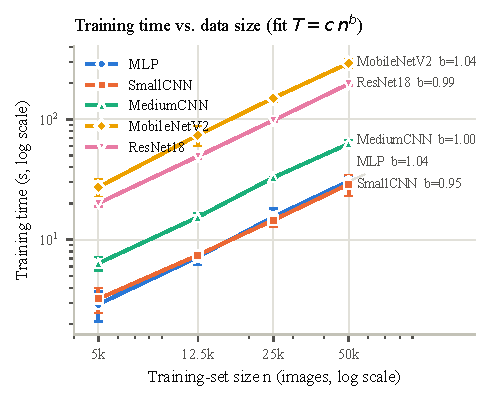
\includegraphics[width=\columnwidth]{fig1_train_time_scaling}
\caption{Training time versus training-set size (log--log, mean $\pm$ std over 5 seeds). Labels give the fitted exponent $b$ of $T=c\,n^b$.}
\label{fig:time}
\end{figure}

\begin{figure}[t]
\centering
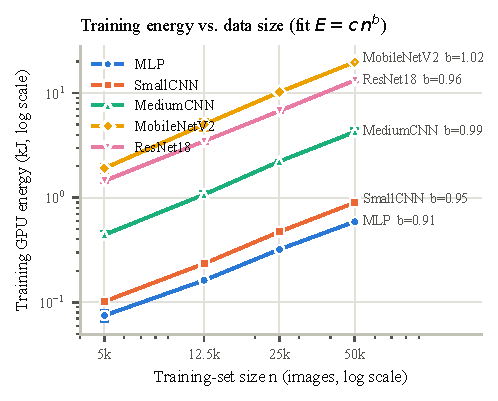
\includegraphics[width=\columnwidth]{fig2_train_energy_scaling}
\caption{Training GPU energy (NVML) versus training-set size (log--log).}
\label{fig:energy}
\end{figure}

\begin{table}[t]
\centering
\caption{Empirical scaling exponents of training time ($b_T$) and GPU energy ($b_E$); theory predicts $b=1$}
\label{tab:scaling}
\resizebox{\columnwidth}{!}{\begin{tabular}{lcccc}
\toprule
Model & $b_T$ [95\% CI] & $R^2_T$ & $b_E$ [95\% CI] & $R^2_E$ \\
\midrule
MLP & 1.041 [0.938, 1.145] & 0.9613 & 0.905 [0.866, 0.944] & 0.9926 \\
SmallCNN & 0.954 [0.861, 1.047] & 0.9628 & 0.949 [0.913, 0.985] & 0.9942 \\
MediumCNN & 1.003 [0.958, 1.049] & 0.9916 & 0.989 [0.951, 1.027] & 0.9939 \\
MobileNetV2 & 1.037 [0.958, 1.115] & 0.9771 & 1.017 [0.967, 1.068] & 0.9899 \\
ResNet18 & 0.991 [0.967, 1.015] & 0.9976 & 0.960 [0.936, 0.985] & 0.9973 \\
\bottomrule
\end{tabular}}
\end{table}

\subsection{Theory versus measurement across models (H2, H4)}
Fig.~\ref{fig:flops} plots measured training time against the theoretical work $6FnE$ (FLOPs). Within each model the
points lie on a straight line, but the lines are shifted: the same number of FLOPs costs very different times for
different architectures. Over the five models the rank correlation between $F$ and training time is only
$\rho=\rhoflops$, and between the parameter count $P$ and time $\rho=\rhoparams$ (neither significant with five
models): neither parameters nor FLOPs alone predict the cost of an architecture. Fig.~\ref{fig:eff}(a) converts
this into achieved throughput: ResNet-18 sustains \tflopsRes{} TFLOP/s and MediumCNN \tflopsMedium{}, but MobileNetV2
only \tflopsMobile{} TFLOP/s, i.e.\ $9\times$ less. As a consequence MobileNetV2, with $6\times$ fewer MACs, trains
in \ttrainMobile\,s compared with \ttrainRes\,s for ResNet-18 at $n=50$k. This is the roofline
prediction~\cite{williams2009roofline}: depthwise convolutions and the six-times-wider, high-resolution expansion
layers move many bytes per FLOP and are bandwidth-bound; in addition MobileNetV2 has 58 weight layers (ResNet-18: 21),
each adding launch overhead. The MLP and SmallCNN reach only \tflopsMlp{} and \tflopsSmall{} TFLOP/s because they are
launch-bound rather than compute-bound, which is why the MLP, with the fewest FLOPs, is not the fastest model. H2 is
therefore confirmed: $F$ orders the convolutional models only coarsely and is not proportional to time.

Fig.~\ref{fig:eff}(b) shows the average GPU power during training. The MLP draws \pavgMlp\,W, barely above the idle
power of \idlepower\,W, and SmallCNN \pavgSmall\,W, while the three larger networks all settle at about 67--68\,W,
the sustained limit of this laptop GPU. GPU utilisation follows the same pattern (MLP \utilMlp\%, ResNet-18
\utilRes\%). Energy is therefore \emph{not} time multiplied by a model-independent constant (H4): for small models
most of the energy is static power spent waiting, so their energy per image is far higher than their FLOPs would
suggest (MLP: \epseMlp\,mJ vs.\ SmallCNN \epseSmall\,mJ per image and epoch, although the MLP does fewer
FLOPs); for large models the GPU is power-saturated and energy becomes proportional to time, so every inefficiency
in throughput---as in MobileNetV2---translates directly into joules.

\begin{figure}[t]
\centering
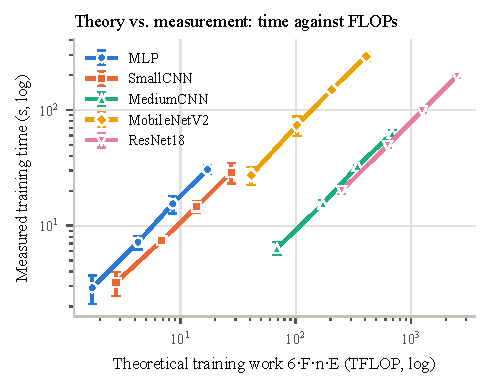
\includegraphics[width=\columnwidth]{fig8_time_vs_flops}
\caption{Measured training time against theoretical training FLOPs ($6FnE$). Each model forms a line with slope $\approx1$, but the offset (efficiency) differs between architectures.}
\label{fig:flops}
\end{figure}

\begin{figure*}[t]
\centering
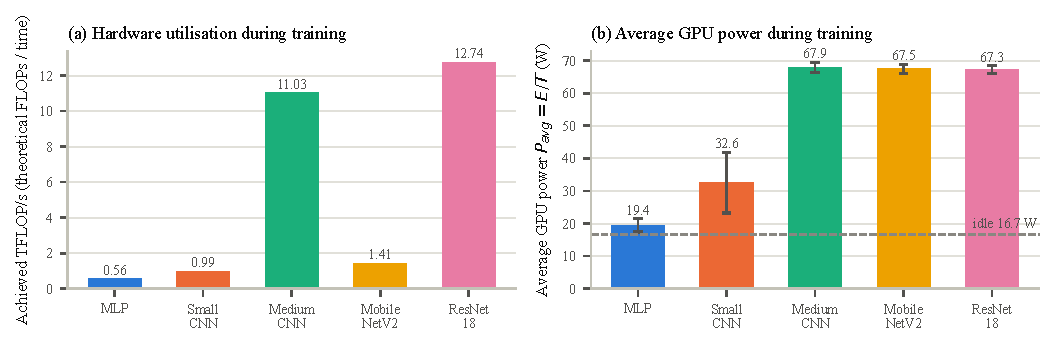
\includegraphics[width=0.85\textwidth]{fig6_efficiency_power}
\caption{(a) Achieved training throughput (theoretical FLOPs / measured time) and (b) average GPU power $P_{avg}=E/T$ at $n=50\,000$. The dashed line marks the idle power of the GPU.}
\label{fig:eff}
\end{figure*}

\subsection{Memory (H3)}
Fig.~\ref{fig:mem} compares the analytical estimate \eqref{eq:mem} with the measured model-attributable peak VRAM.
The two are strongly correlated (Pearson $r=\rvram$). The ranking is set by the activation term, confirming H3:
MobileNetV2, with only $\paramsMobile$M parameters, needs the most VRAM (\vramMobile\,MB) because
$A=\actsMobile$K activations per image are stored for back-propagation, whereas ResNet-18 with $5\times$ more
parameters needs \vramRes\,MB. The MLP has more parameters than MediumCNN but needs only \vramMlp\,MB. The analytical
model under-estimates MobileNetV2 (\vramtheoMobile\,MB), because BatchNorm and ReLU6 inputs and cuDNN workspaces of
the depthwise layers are kept in addition to the layer outputs, and slightly over-estimates ResNet-18
(\vramtheoRes\,MB), whose in-place ReLUs share storage. As predicted, peak VRAM does not depend on $n$: the fitted
exponents of VRAM versus $n$ are below 0.004 for every model (\texttt{scaling\_exponents.csv}). Per image, inference
is far cheaper than training (ResNet-18: \vraminfRes\,MB for a batch of 1000 vs.\ \vramRes\,MB for a batch of 128,
i.e.\ $\approx$0.6 vs.\ 3.2\,MB per image) because no activations, gradients or optimiser states are kept.
Process RAM (710--950\,MB) is dominated by the Python/CUDA runtime and is almost model-independent, because the data
reside on the GPU. This agrees with Iyer \emph{et al.}~\cite{iyer2026greenai}, who also found memory to be an
independent deployment constraint that does not follow parameter count.

\begin{figure}[t]
\centering
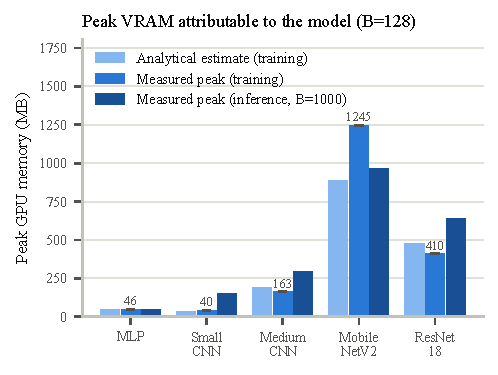
\includegraphics[width=\columnwidth]{fig5_memory_vram}
\caption{Peak GPU memory: analytical estimate of Eq.~(\ref{eq:mem}) versus measurement for training ($B=128$) and inference ($B=1000$).}
\label{fig:mem}
\end{figure}

\subsection{Accuracy and the performance--cost trade-off (H5)}
Fig.~\ref{fig:acc} shows the learning curves. All models improve with $n$, but with diminishing returns: ResNet-18
gains 26 points from 5k to 12.5k images and only 4 points from 25k to 50k, while its cost doubles at each step. The
curves also cross: with 5k images MediumCNN (\accsmallMedium\%) is far better than MobileNetV2 (\accsmallMobile\%)
and ResNet-18 (\accsmallRes\%); the larger networks overtake it only once enough data is available. The
SmallCNN is unstable with 5k images (std 7 points) under the shared learning rate.

Fig.~\ref{fig:pareto} places every model in the accuracy--energy plane at $n=50$k. ResNet-18 achieves the highest
accuracy (\accRes\%$\pm$\accsdRes) and MediumCNN \accMedium\%$\pm$\accsdMedium, a significant difference (Welch
$p<10^{-4}$); but ResNet-18 consumes \egpuRes\,kJ of GPU energy against \egpuMedium\,kJ. The extra \dacc{} accuracy
points therefore cost \denergy\,kJ, i.e.\ \kjperpoint\,kJ per percentage point. MobileNetV2 is dominated: its
accuracy (\accMobile\%) is not significantly different from MediumCNN ($p=0.25$) while it needs $4.6\times$ more
energy, and it is both less accurate and more expensive than ResNet-18. The MLP, despite its \paramsMlp M parameters,
reaches only \accMlp\%, because it ignores the spatial structure of images. The Pareto front---MLP, SmallCNN,
MediumCNN, ResNet-18---is the set from which a practitioner should choose given an energy budget; H5 is confirmed.
Precision, recall and F1 track accuracy closely on this balanced data set (macro F1 within 0.4 points of accuracy),
and macro ROC-AUC exceeds 99\% for the three larger CNNs.

\begin{figure}[t]
\centering
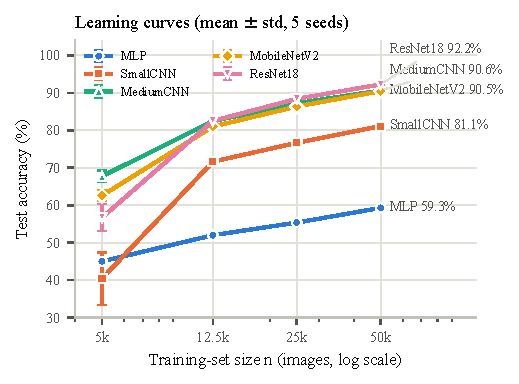
\includegraphics[width=\columnwidth]{fig3_accuracy_vs_n}
\caption{Test accuracy versus training-set size (mean $\pm$ std over 5 seeds).}
\label{fig:acc}
\end{figure}

\begin{figure}[t]
\centering
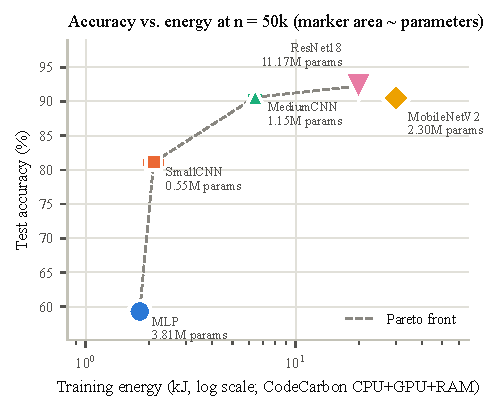
\includegraphics[width=\columnwidth]{fig4_tradeoff_accuracy_energy}
\caption{Accuracy--energy trade-off at $n=50\,000$. Marker area is proportional to $\sqrt{P}$; the dashed line connects the Pareto-optimal models.}
\label{fig:pareto}
\end{figure}

\subsection{Inference: batched vs.\ online, GPU vs.\ CPU}
Fig.~\ref{fig:inf} and Table~\ref{tab:cpugpu} compare the inference settings. In batched GPU mode ResNet-18 classifies
the 10k test images in \tinfRes\,ms (\einfimgRes\,mJ per image), MediumCNN in \tinfMedium\,ms and MobileNetV2 in
\tinfMobile\,ms, again slower than ResNet-18 despite fewer FLOPs. With $B=1$ the online latency follows the
\emph{depth} of the network rather than its FLOPs: \latSmall\,ms (SmallCNN, 4 layers), \latMlp\,ms (MLP, 4),
\latMedium\,ms (MediumCNN, 7), \latRes\,ms (ResNet-18, 21) and \latMobile\,ms (MobileNetV2, 58), because a single image
cannot fill the GPU and every layer costs a roughly fixed kernel-launch time---the same constant term seen in training.
On the CPU, ResNet-18 and MobileNetV2 both need $\approx$5.9\,ms per image, \speedupRes$\times$ and
\speedupMobile$\times$ slower than batched GPU inference, whereas the MLP and SmallCNN need only \cpumsMlp{} and
\cpumsSmall\,ms per image---faster on a CPU batch than a single-image request on the GPU. For small models the CPU is
therefore a sensible deployment target, consistent with the GPU/CPU observations of {\c{C}}etinkaya and
Sertba{\c{s}}~\cite{cetinkaya2022gpucpu} and the embedded-AI perspective of~\cite{zhang2023embedded}.

\begin{figure}[t]
\centering
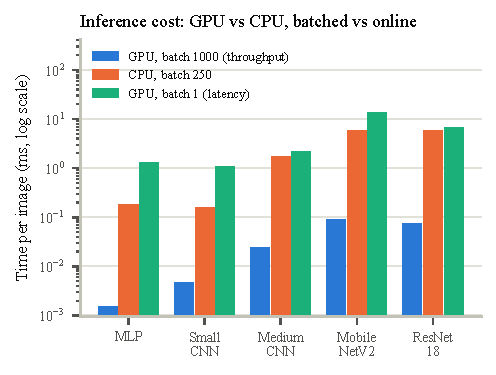
\includegraphics[width=\columnwidth]{fig7_inference}
\caption{Inference time per image: batched GPU ($B=1000$), CPU ($B=250$) and online GPU latency ($B=1$), log scale.}
\label{fig:inf}
\end{figure}

\begin{table}[t]
\centering
\caption{GPU versus CPU inference per image at $n=50\,000$}
\label{tab:cpugpu}
\resizebox{\columnwidth}{!}{\begin{tabular}{lcccc}
\toprule
Model & GPU (ms/img) & CPU (ms/img) & Speed-up & CPU RAM (MB) \\
\midrule
MLP & 0.0015 & 0.186 $\pm$ 0.032 & 125$\times$ & 765 \\
SmallCNN & 0.0048 & 0.157 $\pm$ 0.034 & 33$\times$ & 812 \\
MediumCNN & 0.0247 & 1.744 $\pm$ 0.314 & 70$\times$ & 963 \\
MobileNetV2 & 0.0901 & 5.888 $\pm$ 0.671 & 65$\times$ & 1345 \\
ResNet18 & 0.0748 & 5.893 $\pm$ 1.183 & 79$\times$ & 1149 \\
\bottomrule
\end{tabular}}
\end{table}

\subsection{Carbon footprint}
According to CodeCarbon, the GPU accounts for \sharegpu\% of the training energy, the CPU for \sharecpu\% and the RAM
for \shareram\%; the CodeCarbon GPU estimate agrees with the NVML counter (ratio \ccvsnvml). One full-data
training of ResNet-18 emits \coRes\,g CO$_2$-eq on the Turkish grid, MediumCNN \coMedium\,g and the MLP \coMlp\,g.
The complete study (\nruns{} trainings, \totalhours\,h of training) consumed \totalwh\,Wh and emitted
\totalco\,g CO$_2$-eq. These values are small in absolute terms, but they scale linearly with $n$, $E$ and the
number of hyper-parameter trials, which is why the per-run ratios matter~\cite{strubell2019energy,patterson2021carbon}.

\subsection{Implementation sensitivity}
A preliminary micro-benchmark (supplementary script \texttt{bench\_precision\_\allowbreak layout.py}) showed that the \emph{same} model and the
\emph{same} FLOPs can differ in speed by up to $8.5\times$ depending on numeric precision and memory layout:
float16 with channels-last tensors made MobileNetV2 $\approx$105\,s per epoch and ResNet-18 $\approx$39\,s, whereas
bfloat16 with channels-last made them $\approx$12\,s and $\approx$11\,s. All reported experiments use the fastest configuration for every model (bfloat16,
channels-last). This mirrors the observation of~\cite{akpinar2026dc} that implementation choices can outweigh
asymptotic differences, and is a reminder that constant factors are part of practical complexity.

\subsection{Threats to validity}
(i) All results come from one laptop GPU; absolute values will differ on other hardware, although the scaling
exponents and memory model are hardware-independent. (ii) The CPU energy is a CodeCarbon estimate because RAPL is
not exposed on Windows; GPU energy is a hardware measurement. (iii) A fixed budget of 15 epochs favours fast-converging
models; longer training would raise the accuracy of all CNNs (ResNet-18 typically exceeds 93\%). (iv) Very short
phases ($<2$\,s) are affected by the update period of the energy counter; for inference we therefore repeat passes
for at least 3\,s. (v) All runs share one Python process, so the peak process RAM includes memory cached from
earlier runs; its large standard deviation reflects run order rather than the model, and RAM should be read as an
upper bound.

% ============================================================================
\section{Conclusion and Future Work}
We measured time, memory, energy and accuracy of five DNN architectures on CIFAR-10 over \nruns{} controlled runs and
related them to their analytical complexity. Within an architecture, the theory is accurate: training time grows
linearly with the data size (all exponents compatible with 1), and peak memory is independent of $n$ and follows the
$3\cdot4P + BAb$ model ($r=\rvram$). Across architectures, the operation count $F$ does not determine the cost:
arithmetic intensity, network depth and fixed per-step overheads change the effective constant by an order of
magnitude, so that MobileNetV2 is slower, more memory-hungry and more energy-hungry than a network with six times more
FLOPs, and online latency tracks depth rather than FLOPs. Energy is not a fixed multiple of time: small models waste
static power near idle, and average power drifts with run length, which makes energy scale slightly sub-linearly.
Energy must therefore be measured, not inferred from time. On the accuracy--energy Pareto front, a VGG-style CNN
offers \accMedium\% accuracy for one third of the energy of ResNet-18 (\accRes\%).

Future work includes (i) repeating the protocol on a Linux workstation with RAPL to measure CPU energy directly,
(ii) varying batch size and epochs to study the $B\cdot A$ memory term and time-to-accuracy, (iii) adding
quantisation and pruning~\cite{iyer2026greenai}, and (iv) extending the analysis to Transformers.

\section*{Code and Data Availability}
All source code, raw measurements (\texttt{raw\_runs.csv}) and analysis scripts are provided with this paper.

\bibliographystyle{IEEEtran}
\bibliography{refs}

\end{document}
